A base de dados de expressões faciais utilizada para o desenvolvimento deste trabalho é denominada \emph{Facial Expression Recognition Challenge} (FER2013). Esta base contém $35.887$ imagens faciais em escala de cinza com dimensões de $48\times 48$ pixels, rotuladas de maneira supervisionada segundo uma das sete expressões faciais universais, conforme amostras ilustradas na Figura \ref{fig:samples}. \todo{Incluir os rótulos nestes exemplos}

\begin{figure}[!htb]
    \centering
    \caption{Amostras de imagens faciais e seus respectivos rótulos da base de dados FER2013.} \label{fig:samples}
    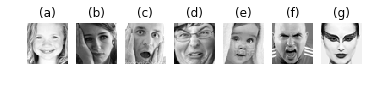
\includegraphics[width=10cm]{images/samples.png}
\end{figure}

Os exemplos disponíveis na FER2013 se distribuem de maneira heterogênea perante as classes consideradas, conforme ilustra o gráfico da Figura \ref{fig:dataset}. O número de exemplos rotulado com a expressão ``nojo'', por exemplo, representam apenas $1.5\%$ do total de exemplos disponíveis. Estas características evidenciam o desbalanceamento do conjunto de dados considerado no tocante à quantidade de amostras por classe. \todo{Rodrigo, veja o gráfico que está na pasta de imagens, intitulado ``boxplot-volumemensal''. Este é o padrão para figuras em artigos científicos. No matplotlib, o set style é \texttt{xtics}. Ajeitar o xlabel para Expressões e o ylabel para Amostras. Consertar todas as demais figuras para este padrão.}

\begin{figure}[!htb]
    \centering
    \caption{Histograma da distribuição de imagens por tipo de expressão facial na base FER2013.}  \label{fig:dataset}
    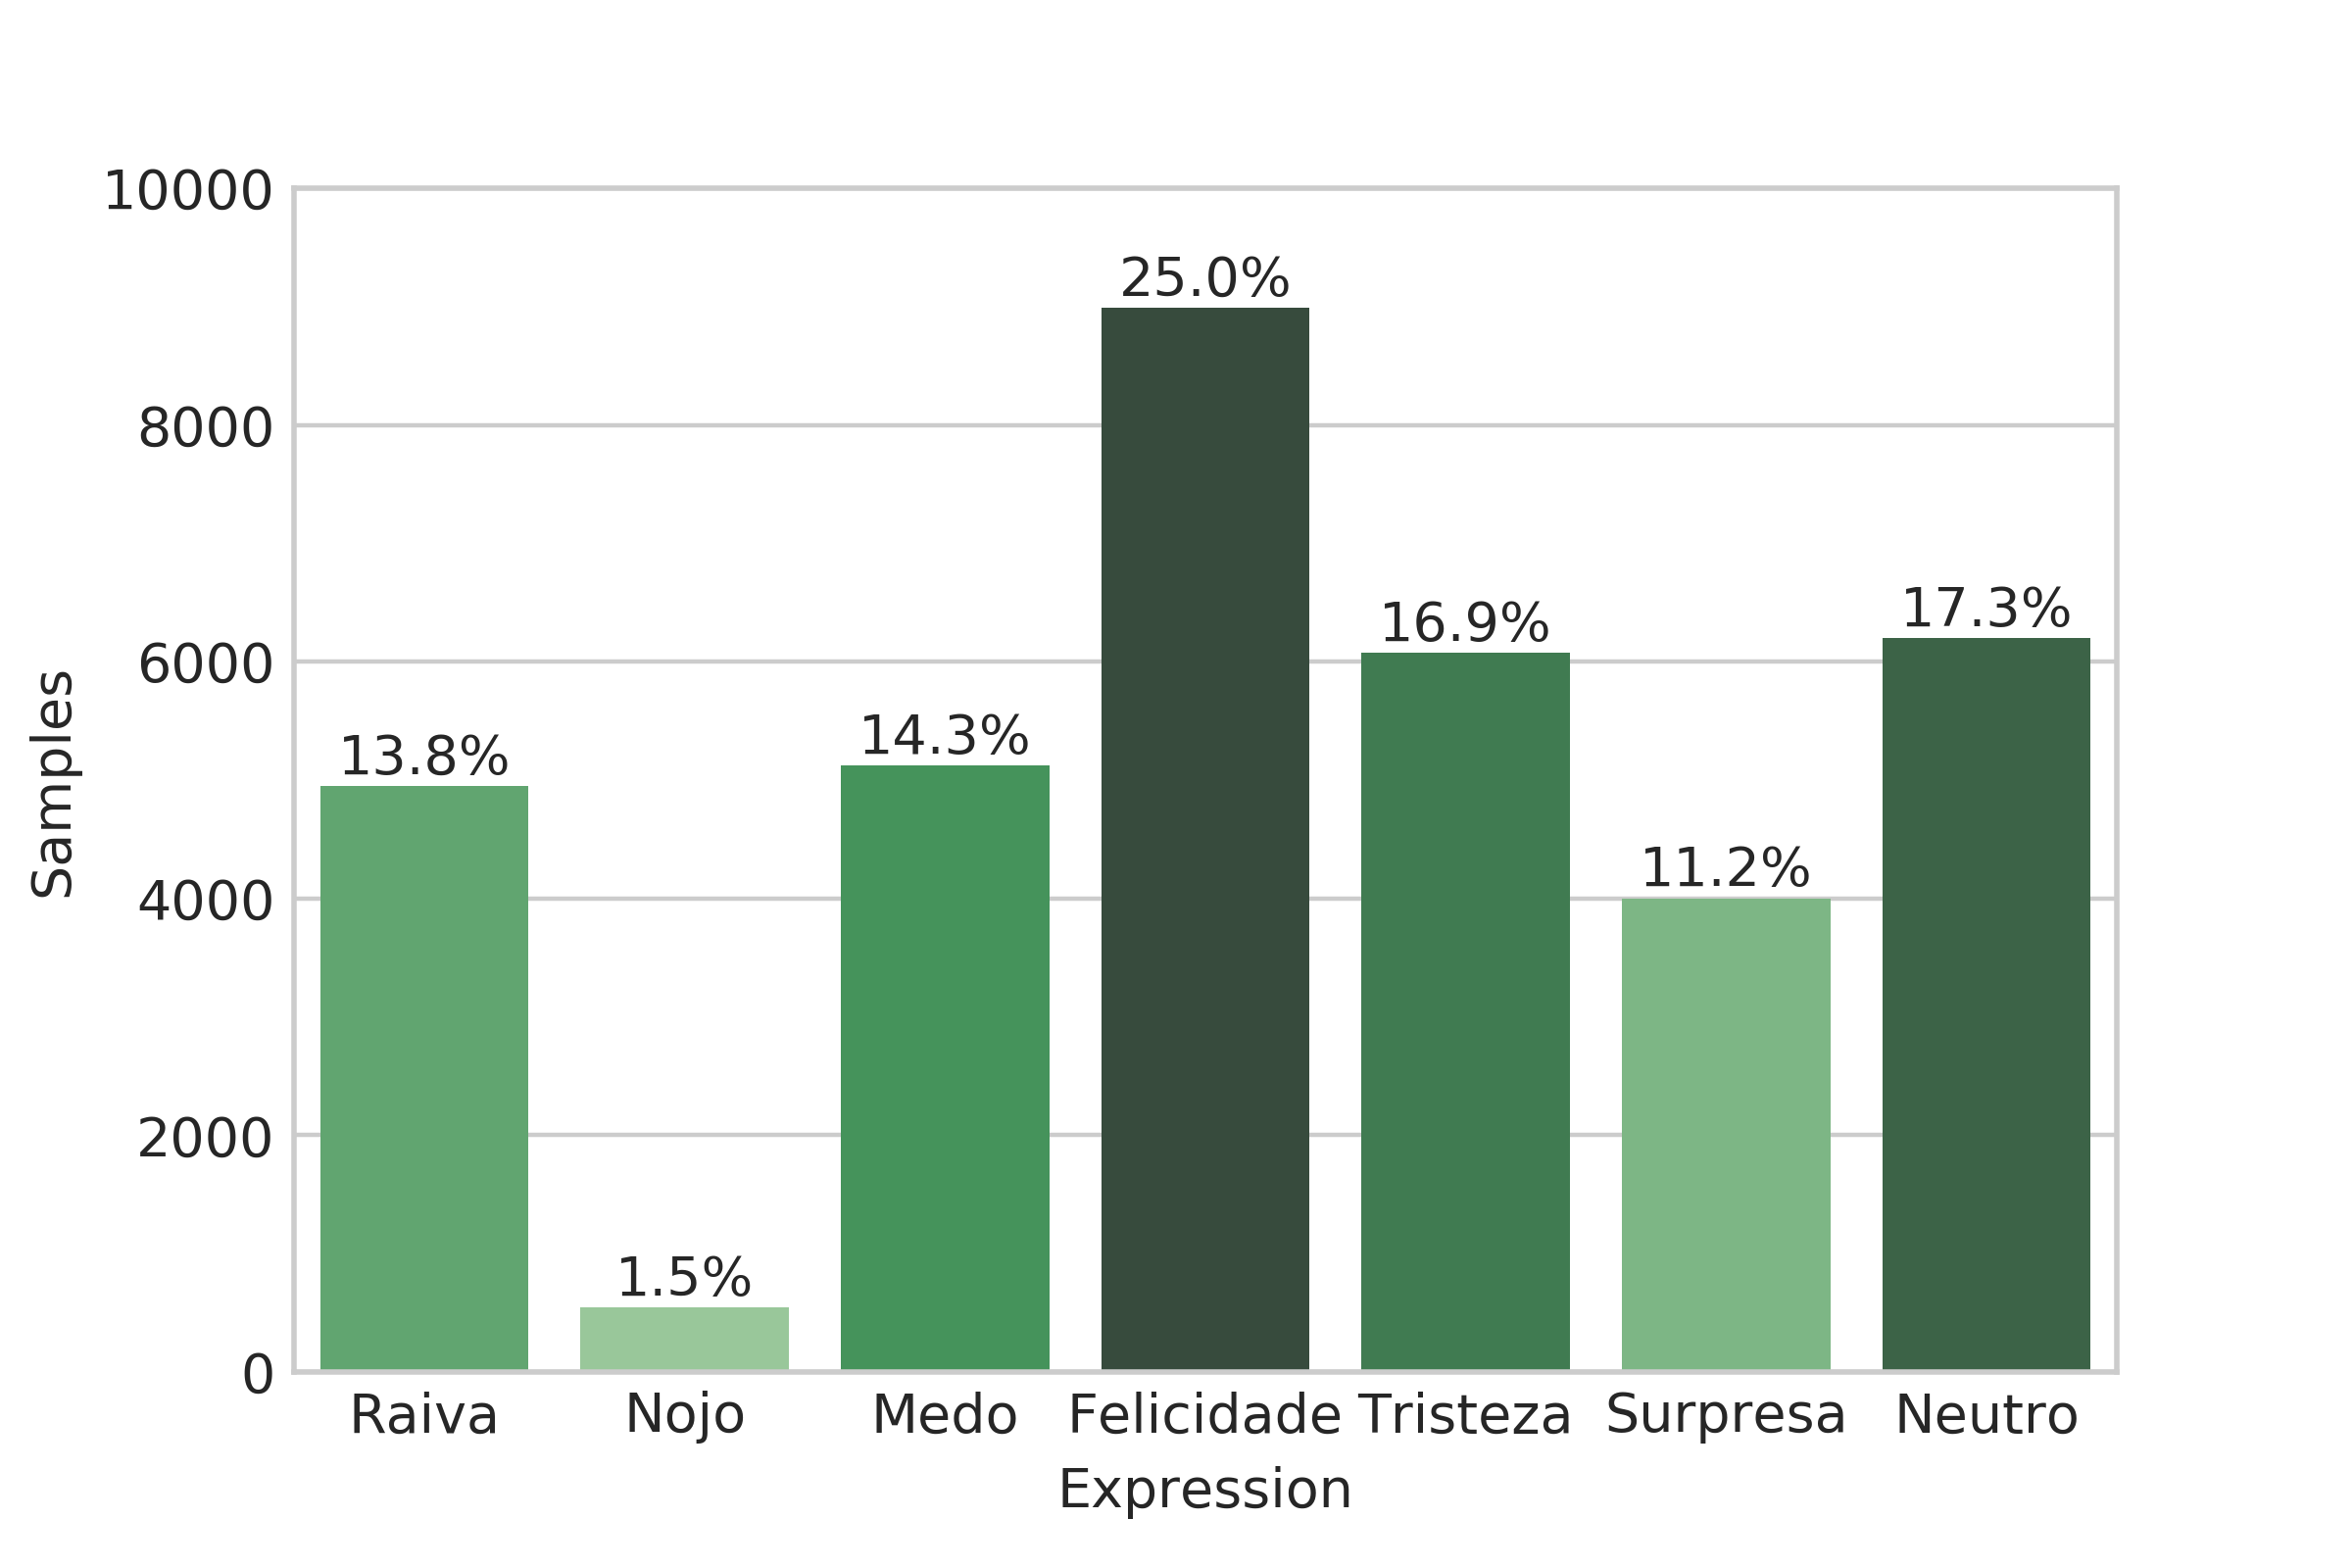
\includegraphics[width=10cm]{images/expression_distribution.png}
\end{figure}



Segundo \cite{}, o tamanho de um modelo de CNN está diretamente relacionado ao tamanho da base de dados, onde quanto maior a quantidade de exemplos, maior pode ser o modelo, pois, em caso contrário, não será possível a geração de modelos com maior complexidade e que possuem melhor taxa de generalização. Visto isto, utilizou-se da técnica \emph{Augmentation} para pseudo expansão da da base de dados.
